\documentclass[tikz, border=12pt]{standalone}
\usepackage{tikz}
\usepackage{amsmath}
\usepackage{amssymb}
\usetikzlibrary{arrows.meta, positioning, fit, backgrounds, calc}

\definecolor{cpuBlue}{RGB}{180,210,240}
\definecolor{cpuPurple}{RGB}{200,190,240}
\definecolor{cpuCoral}{RGB}{240,180,165}
\definecolor{cpuAmber}{RGB}{250,220,160}
\definecolor{cpuTeal}{RGB}{160,225,205}
\definecolor{cpuGray}{RGB}{220,218,210}
\definecolor{bdGray}{RGB}{140,138,130}
\definecolor{loopBg}{RGB}{250,249,246}

\tikzset{
  wide/.style={rectangle, rounded corners=5pt,
    text width=12.5cm, minimum height=1.05cm,
    draw=bdGray, line width=0.4pt, font=\small, align=center},
  blueN/.style={wide, fill=cpuBlue},
  purpleN/.style={wide, fill=cpuPurple},
  coralN/.style={wide, fill=cpuCoral, minimum height=1.5cm, line width=0.8pt},
  amberN/.style={wide, fill=cpuAmber},
  tealN/.style={wide, fill=cpuTeal, text width=8cm},
  grayN/.style={wide, fill=cpuGray, text width=5.8cm},
  eqN/.style={wide, fill=cpuGray, text width=5.6cm, minimum height=1.05cm},
  arr/.style={-{Stealth[length=5pt,width=4pt]}, line width=0.7pt, color=bdGray},
  slabel/.style={font=\footnotesize\itshape, text=bdGray},
  clabel/.style={font=\ttfamily\footnotesize, text=bdGray!80},
}

\begin{document}
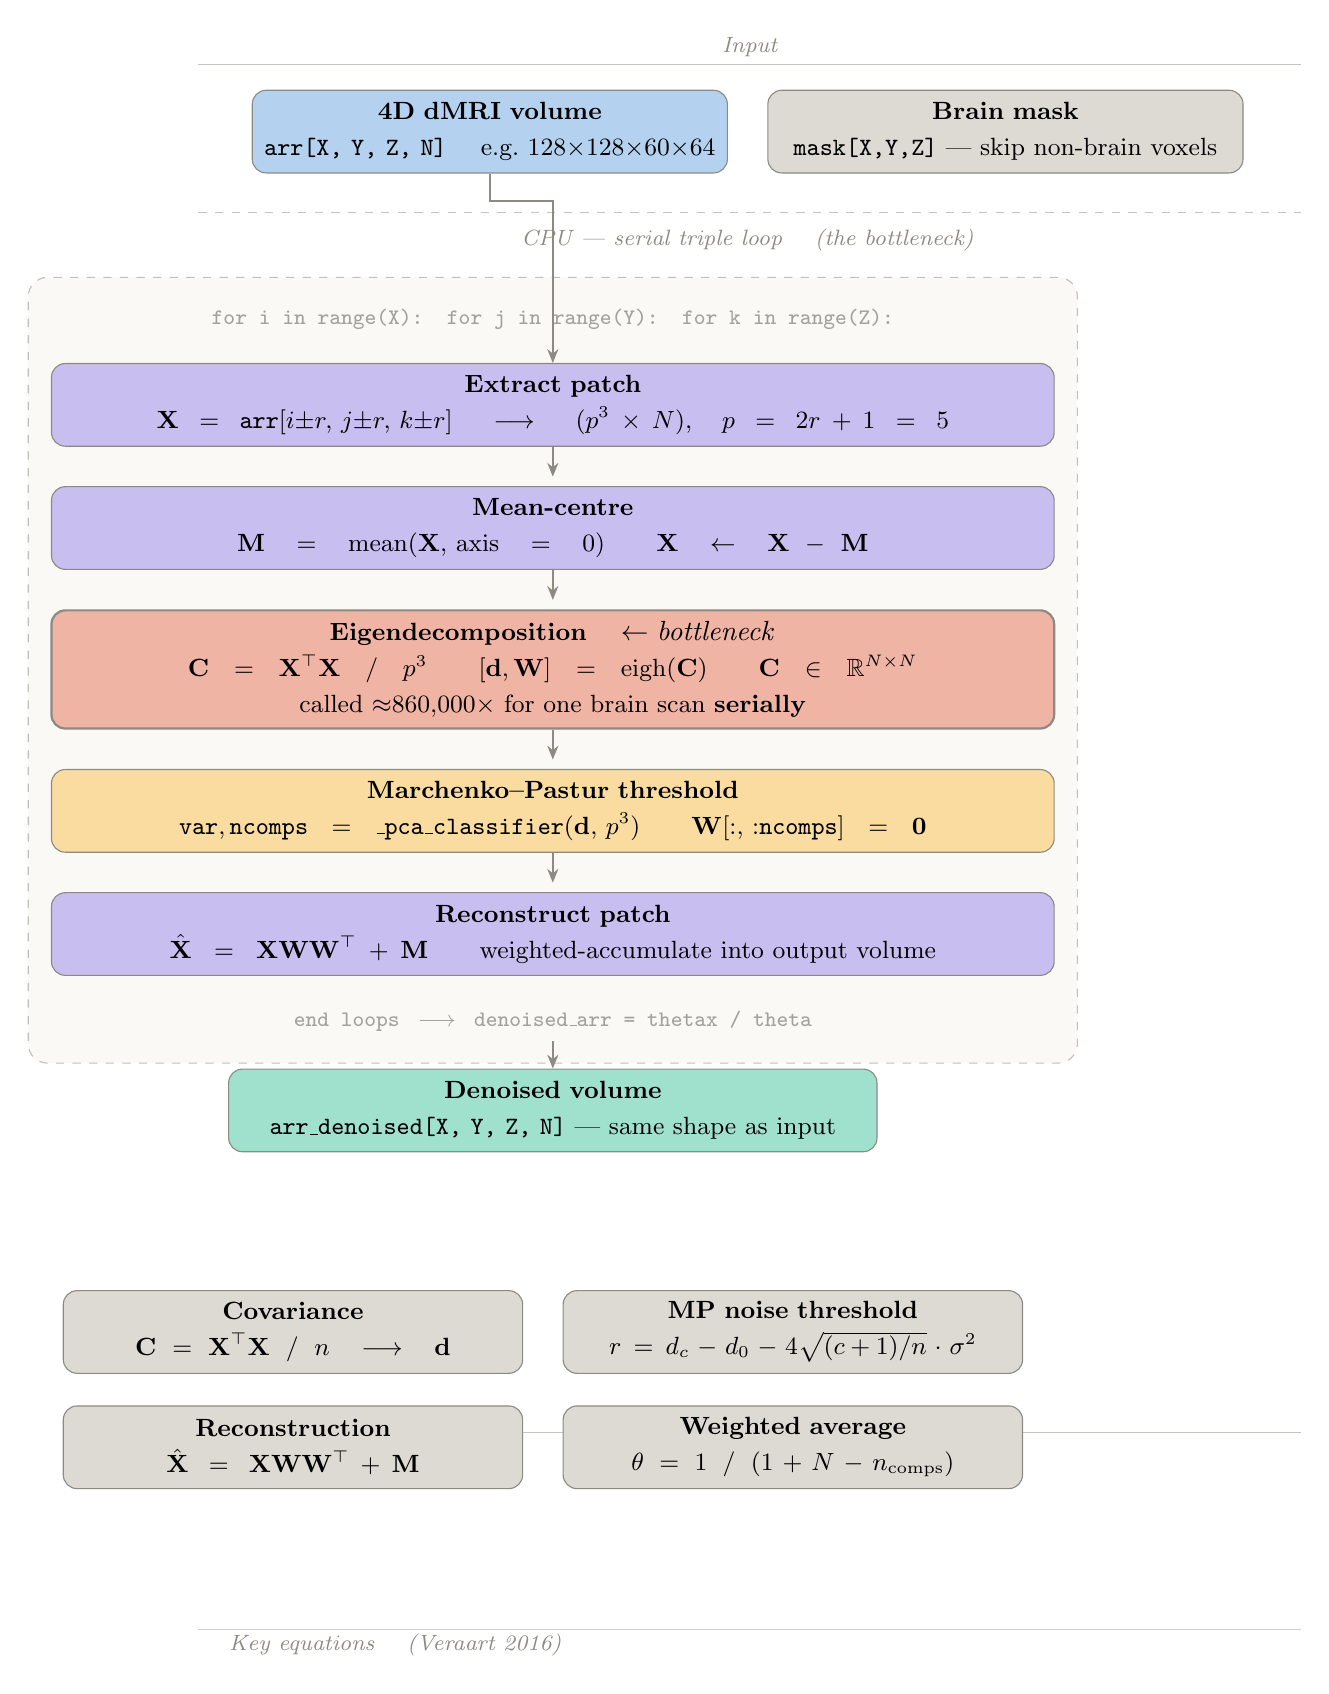
\begin{tikzpicture}[node distance=0.45cm and 0.5cm]

\node[slabel] (L1) at (0,0) {Input};
\draw[bdGray!50, line width=0.3pt] (-7.0,-0.22) -- (7.0,-0.22);

\node[blueN, text width=5.8cm, below=0.3cm of L1, xshift=-3.3cm] (vol)
  {\textbf{4D dMRI volume}\\[2pt]
   \texttt{arr[X, Y, Z, N]} \quad e.g.\ $128{\times}128{\times}60{\times}64$};

\node[grayN, right=0.5cm of vol] (msk)
  {\textbf{Brain mask}\\[2pt]
   \texttt{mask[X,Y,Z]} --- skip non-brain voxels};

\node[slabel, below=0.85cm of vol.south west, anchor=west, xshift=3.3cm] (L2)
  {CPU --- serial triple loop \quad (the bottleneck)};
\draw[bdGray!50, dashed, line width=0.3pt] (-7.0,-2.1) -- (7.0,-2.1);

\node[clabel, below=1.6cm of vol, xshift=0.8cm] (LC)
  {\texttt{for i in range(X):\ \ for j in range(Y):\ \ for k in range(Z):}};

\node[purpleN, below=0.3cm of LC] (S1)
  {\textbf{Extract patch}\\[2pt]
   $\mathbf{X} = \texttt{arr}[i{\pm}r,\,j{\pm}r,\,k{\pm}r]
   \;\longrightarrow\; (p^3 \times N),\quad p=2r+1=5$};
\draw[arr] (S1.south) -- ++(0,-0.38);

\node[purpleN, below=0.5cm of S1] (S2)
  {\textbf{Mean-centre}\\[2pt]
   $\mathbf{M} = \mathrm{mean}(\mathbf{X},\,\text{axis}=0)
   \qquad \mathbf{X} \leftarrow \mathbf{X} - \mathbf{M}$};
\draw[arr] (S2.south) -- ++(0,-0.38);

\node[coralN, below=0.5cm of S2] (S3)
  {\textbf{Eigendecomposition} \quad {\normalsize\textit{$\leftarrow$ bottleneck}}\\[2pt]
   $\mathbf{C} = \mathbf{X}^\top\mathbf{X}\;/\;p^3
   \qquad [\mathbf{d},\mathbf{W}] = \mathrm{eigh}(\mathbf{C})
   \qquad \mathbf{C}\in\mathbb{R}^{N\times N}$\\[2pt]
   called ${\approx}860{,}000\times$ for one brain scan \textbf{serially}};
\draw[arr] (S3.south) -- ++(0,-0.38);

\node[amberN, below=0.5cm of S3] (S4)
  {\textbf{Marchenko--Pastur threshold}\\[2pt]
   $\texttt{var},\texttt{ncomps} = \texttt{\_pca\_classifier}(\mathbf{d},\,p^3)
   \qquad \mathbf{W}[:,\,{:}\texttt{ncomps}] = \mathbf{0}$};
\draw[arr] (S4.south) -- ++(0,-0.38);

\node[purpleN, below=0.5cm of S4] (S5)
  {\textbf{Reconstruct patch}\\[2pt]
   $\hat{\mathbf{X}} = \mathbf{X}\mathbf{W}\mathbf{W}^\top + \mathbf{M}
   \qquad\text{weighted-accumulate into output volume}$};

\node[clabel, below=0.32cm of S5] (LE)
  {\texttt{end loops}
   $\;\longrightarrow\;$ \texttt{denoised\_arr = thetax / theta}};

\begin{pgfonlayer}{background}
  \node[draw=bdGray!55, dashed, fill=loopBg, rounded corners=7pt, inner sep=8pt,
        fit=(LC)(S1)(S2)(S3)(S4)(S5)(LE)] (loopbox) {};
\end{pgfonlayer}

\draw[bdGray!50, line width=0.3pt] (-7.0,-17.6) -- (7.0,-17.6);
\node[slabel] at (-5.5,-17.8) {Output};

\node[tealN, below=0.35cm of LE] (OUT)
  {\textbf{Denoised volume}\\[2pt]
   \texttt{arr\_denoised[X, Y, Z, N]} --- same shape as input};

\draw[arr] (LE.south) -- (OUT.north);
\draw[arr] (vol.south) -- ++(0,-0.35) -| (S1.north);

\draw[bdGray!40, line width=0.3pt] (-7.0,-20.1) -- (7.0,-20.1);
\node[slabel] at (-4.5,-20.3) {Key equations \quad (Veraart 2016)};

\node[eqN, below=1.75cm of OUT, xshift=-3.3cm] (E1)
  {\textbf{Covariance}\\[2pt]
   $\mathbf{C} = \mathbf{X}^\top\mathbf{X}\;/\;n
   \;\longrightarrow\; \mathbf{d}$};

\node[eqN, right=0.5cm of E1] (E2)
  {\textbf{MP noise threshold}\\[2pt]
   $r = d_c - d_0 - 4\sqrt{(c+1)/n}\cdot\sigma^2$};

\node[eqN, below=0.4cm of E1] (E3)
  {\textbf{Reconstruction}\\[2pt]
   $\hat{\mathbf{X}} = \mathbf{X}\mathbf{W}\mathbf{W}^\top + \mathbf{M}$};

\node[eqN, right=0.5cm of E3] (E4)
  {\textbf{Weighted average}\\[2pt]
   $\theta = 1\;/\;(1 + N - n_{\mathrm{comps}})$};

\end{tikzpicture}
\end{document}